\section{Process\-Manager Class Reference}
\label{classProcessManager}\index{ProcessManager@{ProcessManager}}
Inheritance diagram for Process\-Manager:\begin{figure}[H]
\begin{center}
\leavevmode
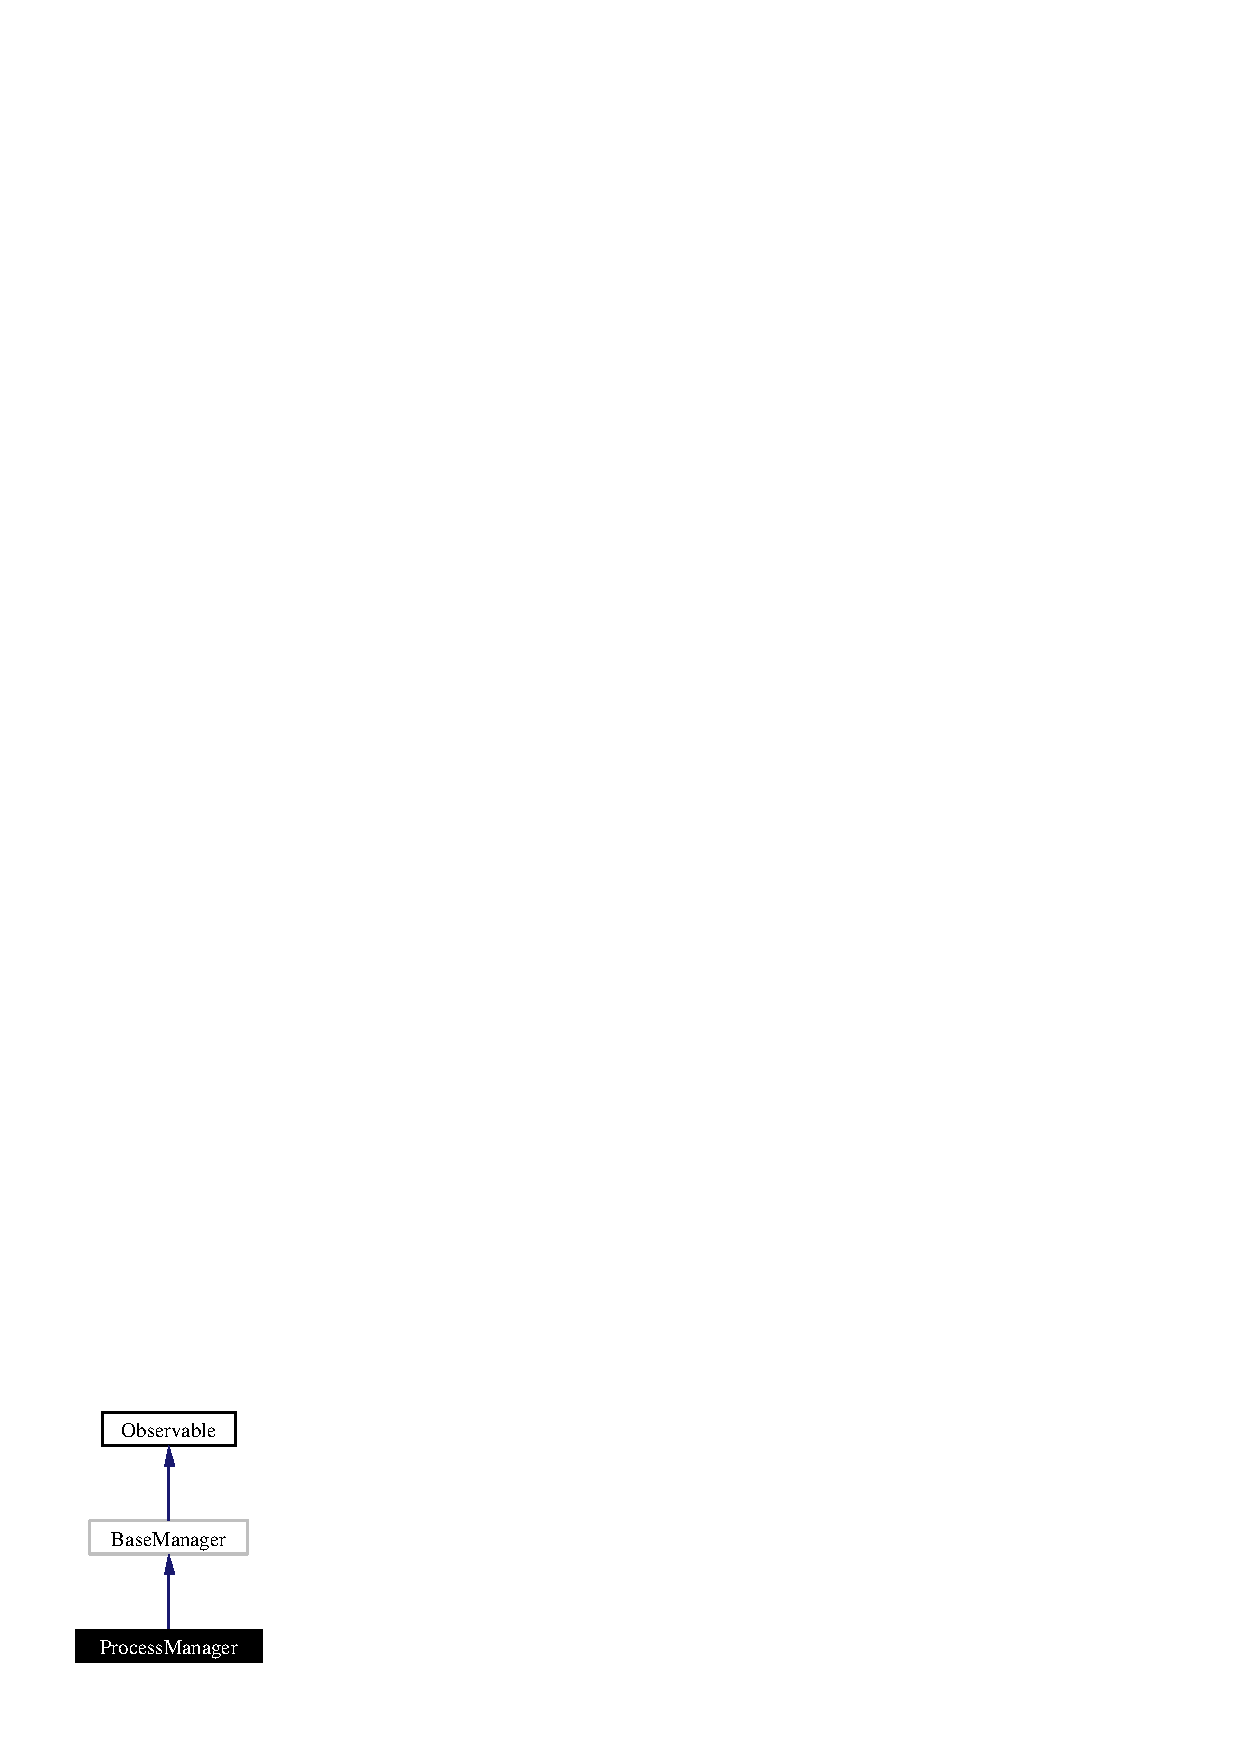
\includegraphics[width=63pt]{classProcessManager__inherit__graph}
\end{center}
\end{figure}
Collaboration diagram for Process\-Manager:\begin{figure}[H]
\begin{center}
\leavevmode
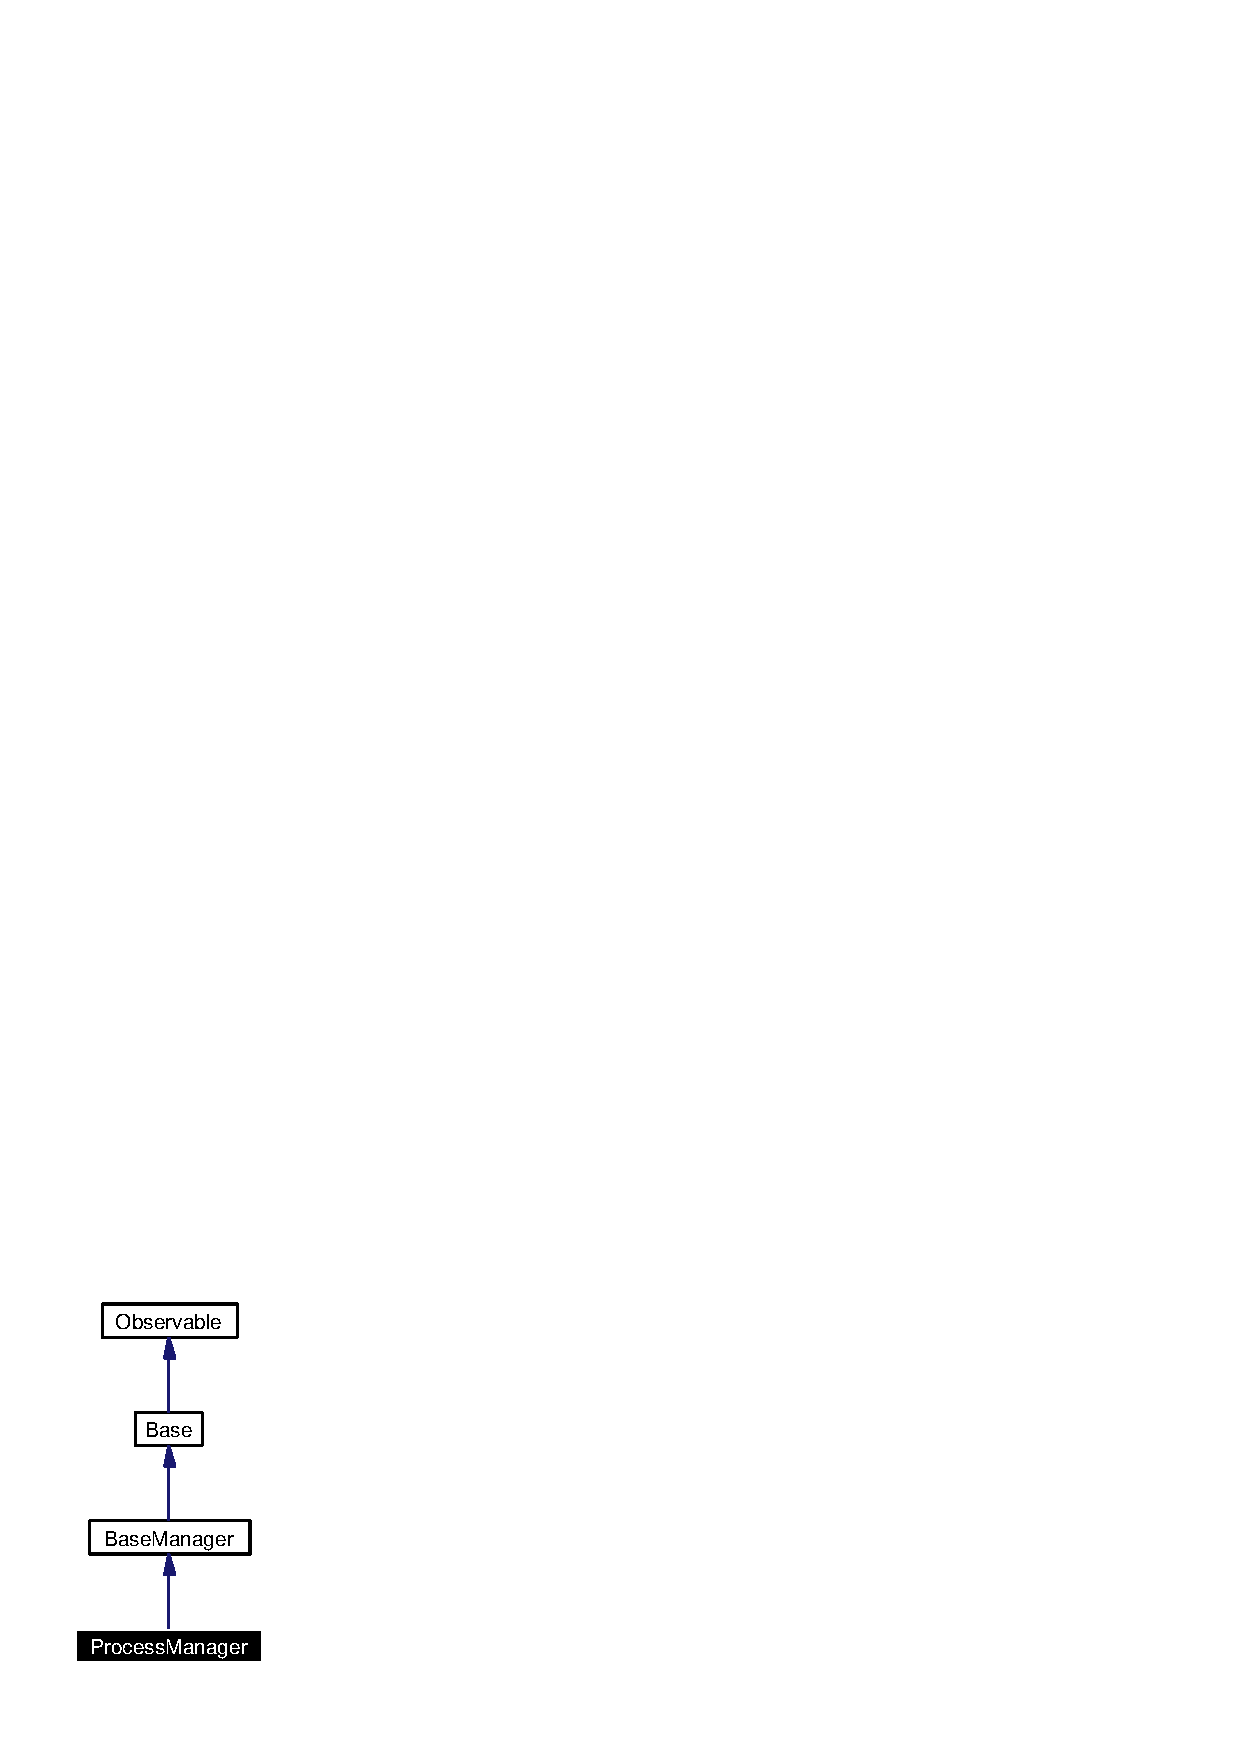
\includegraphics[width=63pt]{classProcessManager__coll__graph}
\end{center}
\end{figure}
\subsection*{Public Member Functions}
\begin{CompactItemize}
\item 
{\bf Process\-Manager} (\$db)
\item 
{\bf activate\_\-process} (\$p\-Id)
\item 
{\bf deactivate\_\-process} (\$p\-Id)
\item 
{\bf new\_\-process\_\-version} (\$p\-Id,\$minor=true)
\item 
{\bf process\_\-name\_\-exists} (\$name,\$version)
\item 
{\bf get\_\-process} (\$p\-Id)
\item 
{\bf list\_\-processes} (\$offset,\$max\-Records,\$sort\_\-mode,\$find,\$where='')
\item 
{\bf remove\_\-process} (\$p\-Id)
\item 
{\bf replace\_\-process} (\$p\-Id,\$vars)
\item 
\index{_rec_copy@{\_\-rec\_\-copy}!ProcessManager@{ProcessManager}}\index{ProcessManager@{ProcessManager}!_rec_copy@{\_\-rec\_\-copy}}
{\bf \_\-rec\_\-copy} (\$dir1,\$dir2)\label{classProcessManager_a9}

\item 
{\bf Process\-Manager} (\$db)
\item 
{\bf activate\_\-process} (\$p\-Id)
\item 
{\bf deactivate\_\-process} (\$p\-Id)
\item 
{\bf serialize\_\-process} (\$p\-Id)
\item 
{\bf unserialize\_\-process} (\$xml)
\item 
{\bf import\_\-process} (\$data)
\item 
{\bf new\_\-process\_\-version} (\$p\-Id,\$minor=true)
\item 
{\bf process\_\-name\_\-exists} (\$name,\$version)
\item 
{\bf get\_\-process} (\$p\-Id)
\item 
{\bf list\_\-processes} (\$offset,\$max\-Records,\$sort\_\-mode,\$find,\$where='')
\item 
{\bf remove\_\-process} (\$p\-Id)
\item 
{\bf replace\_\-process} (\$p\-Id,\$vars)
\item 
\index{_rec_copy@{\_\-rec\_\-copy}!ProcessManager@{ProcessManager}}\index{ProcessManager@{ProcessManager}!_rec_copy@{\_\-rec\_\-copy}}
{\bf \_\-rec\_\-copy} (\$dir1,\$dir2)\label{classProcessManager_a22}

\item 
\index{_start_element_handler@{\_\-start\_\-element\_\-handler}!ProcessManager@{ProcessManager}}\index{ProcessManager@{ProcessManager}!_start_element_handler@{\_\-start\_\-element\_\-handler}}
{\bf \_\-start\_\-element\_\-handler} (\$parser,\$element,\$attribs)\label{classProcessManager_a23}

\item 
\index{_end_element_handler@{\_\-end\_\-element\_\-handler}!ProcessManager@{ProcessManager}}\index{ProcessManager@{ProcessManager}!_end_element_handler@{\_\-end\_\-element\_\-handler}}
{\bf \_\-end\_\-element\_\-handler} (\$parser,\$element)\label{classProcessManager_a24}

\item 
\index{_data_handler@{\_\-data\_\-handler}!ProcessManager@{ProcessManager}}\index{ProcessManager@{ProcessManager}!_data_handler@{\_\-data\_\-handler}}
{\bf \_\-data\_\-handler} (\$parser,\$data)\label{classProcessManager_a25}

\end{CompactItemize}
\subsection*{Public Attributes}
\begin{CompactItemize}
\item 
\index{parser@{parser}!ProcessManager@{ProcessManager}}\index{ProcessManager@{ProcessManager}!parser@{parser}}
{\bf parser}\label{classProcessManager_m0}

\item 
\index{tree@{tree}!ProcessManager@{ProcessManager}}\index{ProcessManager@{ProcessManager}!tree@{tree}}
{\bf tree}\label{classProcessManager_m1}

\item 
\index{current@{current}!ProcessManager@{ProcessManager}}\index{ProcessManager@{ProcessManager}!current@{current}}
{\bf current}\label{classProcessManager_m2}

\item 
\index{buffer@{buffer}!ProcessManager@{ProcessManager}}\index{ProcessManager@{ProcessManager}!buffer@{buffer}}
{\bf buffer}\label{classProcessManager_m3}

\end{CompactItemize}


\subsection{Detailed Description}
This class is used to add,remove,modify and list processes. 



Definition at line 10 of file Process\-Manager/Process\-Manager.php.

\subsection{Constructor \& Destructor Documentation}
\index{ProcessManager@{Process\-Manager}!ProcessManager@{ProcessManager}}
\index{ProcessManager@{ProcessManager}!ProcessManager@{Process\-Manager}}
\subsubsection{\setlength{\rightskip}{0pt plus 5cm}Process\-Manager::Process\-Manager (\$ {\em db})}\label{classProcessManager_a0}


Constructor takes a PEAR::Db object to be used to manipulate roles in the database. 

Definition at line 16 of file Process\-Manager/Process\-Manager.php.\index{ProcessManager@{Process\-Manager}!ProcessManager@{ProcessManager}}
\index{ProcessManager@{ProcessManager}!ProcessManager@{Process\-Manager}}
\subsubsection{\setlength{\rightskip}{0pt plus 5cm}Process\-Manager::Process\-Manager (\$ {\em db})}\label{classProcessManager_a10}


Constructor takes a PEAR::Db object to be used to manipulate roles in the database. 

Definition at line 20 of file src/Process\-Manager/Process\-Manager.php.

\subsection{Member Function Documentation}
\index{ProcessManager@{Process\-Manager}!activate_process@{activate\_\-process}}
\index{activate_process@{activate\_\-process}!ProcessManager@{Process\-Manager}}
\subsubsection{\setlength{\rightskip}{0pt plus 5cm}Process\-Manager::activate\_\-process (\$ {\em p\-Id})}\label{classProcessManager_a11}


Sets a process as active 

Definition at line 32 of file src/Process\-Manager/Process\-Manager.php.\index{ProcessManager@{Process\-Manager}!activate_process@{activate\_\-process}}
\index{activate_process@{activate\_\-process}!ProcessManager@{Process\-Manager}}
\subsubsection{\setlength{\rightskip}{0pt plus 5cm}Process\-Manager::activate\_\-process (\$ {\em p\-Id})}\label{classProcessManager_a1}


Sets a process as active 

Definition at line 28 of file Process\-Manager/Process\-Manager.php.\index{ProcessManager@{Process\-Manager}!deactivate_process@{deactivate\_\-process}}
\index{deactivate_process@{deactivate\_\-process}!ProcessManager@{Process\-Manager}}
\subsubsection{\setlength{\rightskip}{0pt plus 5cm}Process\-Manager::deactivate\_\-process (\$ {\em p\-Id})}\label{classProcessManager_a12}


De-activates a process 

Definition at line 41 of file src/Process\-Manager/Process\-Manager.php.\index{ProcessManager@{Process\-Manager}!deactivate_process@{deactivate\_\-process}}
\index{deactivate_process@{deactivate\_\-process}!ProcessManager@{Process\-Manager}}
\subsubsection{\setlength{\rightskip}{0pt plus 5cm}Process\-Manager::deactivate\_\-process (\$ {\em p\-Id})}\label{classProcessManager_a2}


De-activates a process 

Definition at line 37 of file Process\-Manager/Process\-Manager.php.\index{ProcessManager@{Process\-Manager}!get_process@{get\_\-process}}
\index{get_process@{get\_\-process}!ProcessManager@{Process\-Manager}}
\subsubsection{\setlength{\rightskip}{0pt plus 5cm}Process\-Manager::get\_\-process (\$ {\em p\-Id})}\label{classProcessManager_a18}


Gets a process by p\-Id. Fields are returned as an asociative array 

Definition at line 343 of file src/Process\-Manager/Process\-Manager.php.\index{ProcessManager@{Process\-Manager}!get_process@{get\_\-process}}
\index{get_process@{get\_\-process}!ProcessManager@{Process\-Manager}}
\subsubsection{\setlength{\rightskip}{0pt plus 5cm}Process\-Manager::get\_\-process (\$ {\em p\-Id})}\label{classProcessManager_a5}


Gets a process by p\-Id. Fields are returned as an asociative array 

Definition at line 102 of file Process\-Manager/Process\-Manager.php.

Referenced by import\_\-process(), new\_\-process\_\-version(), replace\_\-process(), and serialize\_\-process().\index{ProcessManager@{Process\-Manager}!import_process@{import\_\-process}}
\index{import_process@{import\_\-process}!ProcessManager@{Process\-Manager}}
\subsubsection{\setlength{\rightskip}{0pt plus 5cm}Process\-Manager::import\_\-process (\$ {\em data})}\label{classProcessManager_a15}


Creates a process from the process data structure, if you want to convert an XML to a process then use first unserialize\_\-process and then this method. 

Definition at line 217 of file src/Process\-Manager/Process\-Manager.php.

References get\_\-process(), and replace\_\-process().\index{ProcessManager@{Process\-Manager}!list_processes@{list\_\-processes}}
\index{list_processes@{list\_\-processes}!ProcessManager@{Process\-Manager}}
\subsubsection{\setlength{\rightskip}{0pt plus 5cm}Process\-Manager::list\_\-processes (\$ {\em offset}, \$ {\em max\-Records}, \$ {\em sort\_\-mode}, \$ {\em find}, \$ {\em where} = '')}\label{classProcessManager_a19}


Lists processes (all processes) 

Definition at line 355 of file src/Process\-Manager/Process\-Manager.php.\index{ProcessManager@{Process\-Manager}!list_processes@{list\_\-processes}}
\index{list_processes@{list\_\-processes}!ProcessManager@{Process\-Manager}}
\subsubsection{\setlength{\rightskip}{0pt plus 5cm}Process\-Manager::list\_\-processes (\$ {\em offset}, \$ {\em max\-Records}, \$ {\em sort\_\-mode}, \$ {\em find}, \$ {\em where} = '')}\label{classProcessManager_a6}


Lists processes (all processes) 

Definition at line 114 of file Process\-Manager/Process\-Manager.php.\index{ProcessManager@{Process\-Manager}!new_process_version@{new\_\-process\_\-version}}
\index{new_process_version@{new\_\-process\_\-version}!ProcessManager@{Process\-Manager}}
\subsubsection{\setlength{\rightskip}{0pt plus 5cm}Process\-Manager::new\_\-process\_\-version (\$ {\em p\-Id}, \$ {\em minor} = true)}\label{classProcessManager_a16}


Creates a new process based on an existing process changing the process version. By default the process is created as an unactive process and the version is by default a minor version of the process.

\begin{Desc}
\item[{\bf Todo}]copy process activities and so \end{Desc}


Definition at line 291 of file src/Process\-Manager/Process\-Manager.php.

References get\_\-process(), and replace\_\-process().\index{ProcessManager@{Process\-Manager}!new_process_version@{new\_\-process\_\-version}}
\index{new_process_version@{new\_\-process\_\-version}!ProcessManager@{Process\-Manager}}
\subsubsection{\setlength{\rightskip}{0pt plus 5cm}Process\-Manager::new\_\-process\_\-version (\$ {\em p\-Id}, \$ {\em minor} = true)}\label{classProcessManager_a3}


Creates a new process based on an existing process changing the process version. By default the process is created as an unactive process and the version is by default a minor version of the process.

\begin{Desc}
\item[{\bf Todo}]copy process activities and so \end{Desc}


Definition at line 50 of file Process\-Manager/Process\-Manager.php.

References get\_\-process(), and replace\_\-process().\index{ProcessManager@{Process\-Manager}!process_name_exists@{process\_\-name\_\-exists}}
\index{process_name_exists@{process\_\-name\_\-exists}!ProcessManager@{Process\-Manager}}
\subsubsection{\setlength{\rightskip}{0pt plus 5cm}Process\-Manager::process\_\-name\_\-exists (\$ {\em name}, \$ {\em version})}\label{classProcessManager_a17}


This function can be used to check if a process name exists, note that this is NOT used by replace\_\-process since that function can be used to create new versions of an existing process. The application must use this method to ensure that processes have unique names. 

Definition at line 333 of file src/Process\-Manager/Process\-Manager.php.\index{ProcessManager@{Process\-Manager}!process_name_exists@{process\_\-name\_\-exists}}
\index{process_name_exists@{process\_\-name\_\-exists}!ProcessManager@{Process\-Manager}}
\subsubsection{\setlength{\rightskip}{0pt plus 5cm}Process\-Manager::process\_\-name\_\-exists (\$ {\em name}, \$ {\em version})}\label{classProcessManager_a4}


This function can be used to check if a process name exists, note that this is NOT used by replace\_\-process since that function can be used to create new versions of an existing process. The application must use this method to ensure that processes have unique names. 

Definition at line 92 of file Process\-Manager/Process\-Manager.php.\index{ProcessManager@{Process\-Manager}!remove_process@{remove\_\-process}}
\index{remove_process@{remove\_\-process}!ProcessManager@{Process\-Manager}}
\subsubsection{\setlength{\rightskip}{0pt plus 5cm}Process\-Manager::remove\_\-process (\$ {\em p\-Id})}\label{classProcessManager_a20}


Removes a process by p\-Id 

Definition at line 387 of file src/Process\-Manager/Process\-Manager.php.\index{ProcessManager@{Process\-Manager}!remove_process@{remove\_\-process}}
\index{remove_process@{remove\_\-process}!ProcessManager@{Process\-Manager}}
\subsubsection{\setlength{\rightskip}{0pt plus 5cm}Process\-Manager::remove\_\-process (\$ {\em p\-Id})}\label{classProcessManager_a7}


Removes a process by p\-Id 

Definition at line 146 of file Process\-Manager/Process\-Manager.php.\index{ProcessManager@{Process\-Manager}!replace_process@{replace\_\-process}}
\index{replace_process@{replace\_\-process}!ProcessManager@{Process\-Manager}}
\subsubsection{\setlength{\rightskip}{0pt plus 5cm}Process\-Manager::replace\_\-process (\$ {\em p\-Id}, \$ {\em vars})}\label{classProcessManager_a21}


Updates or inserts a new process in the database, \$vars is an asociative array containing the fields to update or to insert as needed. \$p\-Id is the process\-Id 

Definition at line 420 of file src/Process\-Manager/Process\-Manager.php.

References get\_\-process().\index{ProcessManager@{Process\-Manager}!replace_process@{replace\_\-process}}
\index{replace_process@{replace\_\-process}!ProcessManager@{Process\-Manager}}
\subsubsection{\setlength{\rightskip}{0pt plus 5cm}Process\-Manager::replace\_\-process (\$ {\em p\-Id}, \$ {\em vars})}\label{classProcessManager_a8}


Updates or inserts a new process in the database, \$vars is an asociative array containing the fields to update or to insert as needed. \$p\-Id is the process\-Id 

Definition at line 178 of file Process\-Manager/Process\-Manager.php.

References get\_\-process().

Referenced by import\_\-process(), and new\_\-process\_\-version().\index{ProcessManager@{Process\-Manager}!serialize_process@{serialize\_\-process}}
\index{serialize_process@{serialize\_\-process}!ProcessManager@{Process\-Manager}}
\subsubsection{\setlength{\rightskip}{0pt plus 5cm}Process\-Manager::serialize\_\-process (\$ {\em p\-Id})}\label{classProcessManager_a13}


Creates an XML representation of a process. 

Definition at line 50 of file src/Process\-Manager/Process\-Manager.php.

References get\_\-process().\index{ProcessManager@{Process\-Manager}!unserialize_process@{unserialize\_\-process}}
\index{unserialize_process@{unserialize\_\-process}!ProcessManager@{Process\-Manager}}
\subsubsection{\setlength{\rightskip}{0pt plus 5cm}Process\-Manager::unserialize\_\-process (\$ {\em xml})}\label{classProcessManager_a14}


Creates a process from its XML representation 

Definition at line 121 of file src/Process\-Manager/Process\-Manager.php.

The documentation for this class was generated from the following files:\begin{CompactItemize}
\item 
Process\-Manager/Process\-Manager.php\item 
src/Process\-Manager/Process\-Manager.php\end{CompactItemize}
